\documentclass[conference]{IEEEtran}
\usepackage[T1]{fontenc}
\usepackage{graphicx,amsmath,booktabs,url,tikz}
\usepackage[hidelinks]{hyperref}
\usetikzlibrary{arrows.meta,positioning}
\graphicspath{{figures/}}
\newcommand{\nei}{not enough information}
\title{Evidence-Grounded Clinical Criterion Screening with a Small Adapted Transformer}
\author{\IEEEauthorblockN{Aaiz Ur Rehman Kazmi}
\IEEEauthorblockA{Roll No. 23I-0589\\Generative AI, Section A\\FAST-NUCES}}
\begin{document}
\maketitle
\begin{abstract}
This educational system predicts clinical-trial criterion labels and patient-sentence evidence using a LoRA-adapted Qwen2.5-1.5B-Instruct model. A fixed patient-grouped split contains 37 training, eight validation, and eight test patients. Saved pure-greedy evaluations show test accuracy improving from 0.155 to 0.704 and evidence micro-F1 from 0.147 to 0.500. Independent implementations demonstrate cache-aware generation, tiled online-softmax attention, and greedy speculative decoding. Recorded GPU experiments show near-constant cached decoding throughput, substantially reduced attention intermediate memory, and slower speculative generation despite token equality. A browser application exposes evidence, exports reports, and adds explicitly identified review rules. Results are limited by small patient counts, label imbalance, incomplete experiment provenance, and unresolved clinical reasoning errors. The system is not an enrollment decision tool.
\end{abstract}
\begin{IEEEkeywords}
clinical trial screening, evidence retrieval, LoRA, KV cache, online softmax, speculative decoding
\end{IEEEkeywords}

\section{Introduction}
Clinical eligibility criteria combine explicit facts, missing information, negation, and numerical limits. A useful screening prototype must distinguish a contradicted criterion from one that cannot be assessed. It must also identify the patient text supporting its answer. This project formulates screening as one patient--criterion decision at a time, followed by transparent aggregation in a browser application. The aggregate is not a separately annotated prediction task.

The contribution is an integrated educational implementation: supervised adaptation on the prescribed dataset, structured evidence outputs, explicit inference algorithms, and a working interface. The objective is reproducible investigation on accessible hardware, not a claim of clinical reliability or improved state-of-the-art performance.

\section{Related Work and Design Alternatives}
TrialGPT studies retrieval, criterion matching, and ranking \cite{trialgpt}. The present project addresses criterion matching using the common annotations rather than reproducing the original end-to-end system. Its published performance is not directly comparable to this small-model, patient-split experiment.

Transformers use attention to contextualize tokens \cite{attention}. An autoregressive decoder is appropriate here because the output includes both a category and a variable-length evidence list. LoRA freezes base weights while learning low-rank updates \cite{lora}; this reduces trainable state but does not remove activation or base-weight memory. Full fine-tuning would require substantially more optimizer storage. Quantization was not used in the recorded final training configuration, reducing complexity in the custom decoding paths.

FlashAttention motivates tiled computation and stable online normalization \cite{flash}. Our implementation retains the mathematical recurrence, but Python loops do not reproduce a fused CUDA kernel's hardware efficiency. Speculative decoding uses a cheaper proposal model and target verification \cite{spec}; our implementation covers the deterministic greedy case, not distribution-preserving stochastic sampling.

\begin{table}[t]
\caption{Documented model alternatives; only Qwen was trained here. Weight memory is an analytical FP16 estimate, excluding caches, activations, and optimizer state.}
\label{tab:models}\centering\small
\begin{tabular}{lcc}\toprule
Property & Qwen2.5-1.5B & SmolLM2-1.7B\\\midrule
Parameters & 1.54B & approximately 1.7B\\
Decoder layers & 28 & 24\\
Query / KV heads & 12 / 2 & 32 / 32\\
Hidden width & 1536 & 2048\\
Context positions & 32768 & 8192\\
Weight memory & 3.08 GB & 3.4 GB\\
License & Apache 2.0 & Apache 2.0\\\bottomrule
\end{tabular}
\end{table}

Table~\ref{tab:models} compares two feasible open-weight instruction decoders using their official cards and configuration \cite{qwen,smol,smolconfig}. Qwen uses RoPE, RMSNorm, SwiGLU, grouped-query attention, and tied embeddings. The cached configuration has a 151936-entry embedding vocabulary. SmolLM2 uses a Llama-family decoder and a 49152-entry vocabulary. Both use their own tokenizer and chat template; token IDs cannot be exchanged between families. Qwen is attractive because its 0.5B family member provides a draft whose vocabulary and EOS token are checked explicitly. Its smaller number of KV heads also lowers cache growth. These are feasibility arguments, not a measured head-to-head accuracy comparison. The alternative comparison was documented during finalization, rather than established as a historical experiment.

\section{Materials and Methods}
\subsection{Dataset and Input Processing}
The sole supervised source is \texttt{ncbi/TrialGPT-Criterion-Annotations}: 1015 rows from 53 patients. Sorted unique patient IDs are shuffled with NumPy \texttt{default\_rng(42)}, then assigned 37/8/8 to train/validation/test, yielding 603/206/206 rows. The published manifest records IDs and counts. Tests verify disjoint patient sets and exclusion of GPT-4-generated columns from prompts.

Notes retain numbered sentence IDs. Each prompt contains a system instruction, numbered patient sentences, the criterion type and text, and permitted labels. Inclusion labels are included, not included, \nei{}, and not applicable; exclusion labels replace the first two with excluded and not excluded. The target is JSON containing a label and integer evidence IDs. A parser rejects malformed JSON, labels outside the type's vocabulary, and out-of-range evidence IDs. It accepts an empty evidence list, so syntactic validity is not a guarantee of grounding.

Training truncation removes trailing sentences to reserve answer tokens; metadata records whether annotated evidence is lost. The repository's recorded summary reports a maximum prompt length of 567 tokens and no truncation at 1024. That summary has not been independently regenerated in this finalization. The app uses a 2048-token budget and reports truncation. A single oversized sentence can exceed the current sentence-removal budget and remains a known edge case.

\begin{figure}[t]\centering
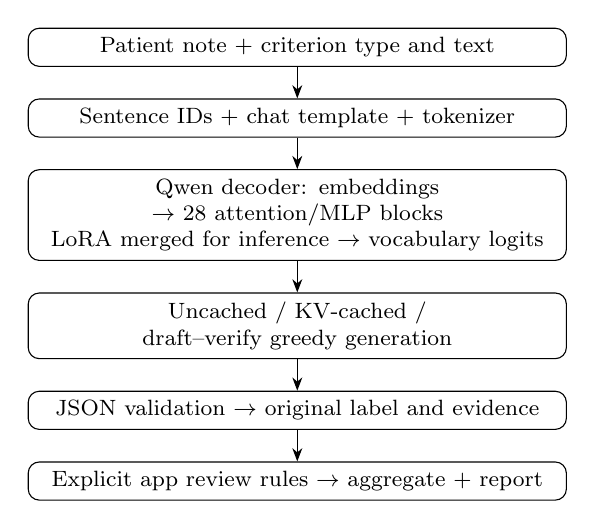
\begin{tikzpicture}[node distance=4mm, every node/.style={draw,rounded corners,align=center,font=\footnotesize,text width=6.6cm},>=Stealth]
\node (a) {Patient note + criterion type and text};
\node[below=of a] (b) {Sentence IDs + chat template + tokenizer};
\node[below=of b] (c) {Qwen decoder: embeddings $\rightarrow$ 28 attention/MLP blocks\\LoRA merged for inference $\rightarrow$ vocabulary logits};
\node[below=of c] (d) {Uncached / KV-cached / draft--verify greedy generation};
\node[below=of d] (e) {JSON validation $\rightarrow$ original label and evidence};
\node[below=of e] (f) {Explicit app review rules $\rightarrow$ aggregate + report};
\draw[->] (a)--(b);\draw[->] (b)--(c);\draw[->] (c)--(d);\draw[->] (d)--(e);\draw[->] (e)--(f);
\end{tikzpicture}
\caption{Application and model workflow. Saved task metrics evaluate the raw parsed output before the application review rules.}\label{fig:flow}
\end{figure}

\subsection{Supervised Adaptation}
For a projection matrix, LoRA learns $\Delta W=(\alpha/r)BA$ while the original $W$ is frozen. Rank 16, scale 32, and dropout 0.05 are applied to query, key, value, output, gate, up, and down projections. Answer-only cross-entropy masks prompt and padding positions with $-100$. Training uses AdamW, learning rate $2\times10^{-4}$, weight decay 0.01, 5\% warmup, cosine decay, gradient clipping at 1.0, FP16 autocast, and gradient scaling.

The balanced run uses three epochs, microbatch two, accumulation eight, seed 42, and gradient checkpointing. Rare criterion-type/label groups are repeated toward 80 rows with a fourfold cap. Repetition increases exposure rather than independent patient diversity. Nominal effective batch size is 16; the final incomplete accumulation group is smaller. The script still divides that group's loss by eight, an implementation limitation of the recorded run.

Validation loss after epochs one, two, and three is 0.1517, 0.1265, and 0.1377. Thus the lowest-loss checkpoint is epoch two, while the selected application adapter is balanced epoch three. Existing task evaluations favor epoch three over epoch two in macro-F1 (0.525 versus 0.515 under the older evaluation setup). The unbalanced epoch-three run gives 0.486. These comparisons support investigating oversampling, but decoding settings in older metric files are incompletely recorded and must not be merged with the final pure-greedy series. Figure~\ref{fig:training} visualizes the saved logs.

\begin{figure}[t]\centering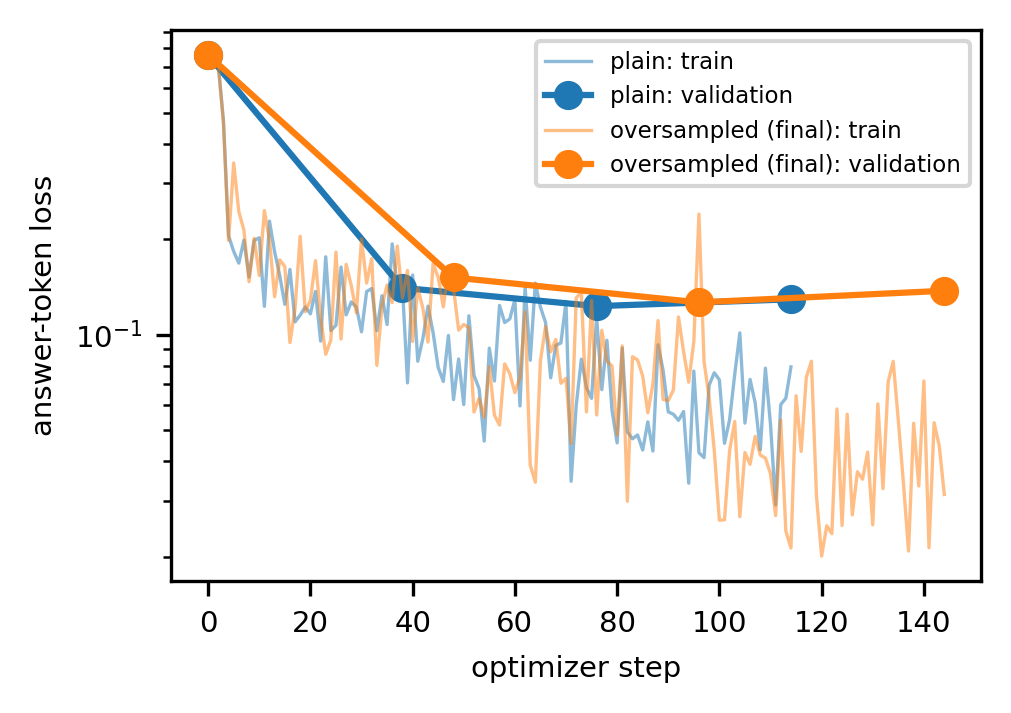
\includegraphics[width=\columnwidth]{training_curves.png}
\caption{Saved training/validation curves for unbalanced and oversampled runs. Lower training loss does not establish stronger criterion reasoning.}\label{fig:training}\end{figure}

\subsection{Explicit KV-Cached Generation}
The uncached path feeds the growing prefix on every step. The cached path prefills all prompt positions once, then feeds only the most recent token with absolute position IDs and cache positions. With prompt length $n$ and $T$ generated tokens, the normal cached path stores $n+T-1$ positions because the final output token is not fed back. A decode query can attend to all stored keys; prefill needs a causal mask.

For $L$ layers, $H_{kv}$ KV heads, head width $d$, and $b$ bytes per scalar, cache storage grows by $2LH_{kv}db$ bytes per token. For this target in FP16, this is $2(28)(2)(128)(2)=28672$ bytes. The implementation is batch-one without padding. Different matrix shapes can change rounding and occasionally flip an argmax near a tie.

\subsection{Tiled Online Softmax}
Reference attention computes $\operatorname{softmax}(QK^T/\sqrt d+M)V$. For each query tile, the implementation streams key tiles and keeps a running maximum $m$, normalizer $l$, and weighted accumulator $A$. Given new tile scores $S$, it updates
\begin{align}
m'&=\max(m,\operatorname{rowmax}(S)),\\
P&=\exp(S-m'),\quad \alpha=\exp(m-m'),\\
l'&=\alpha l+\operatorname{rowsum}(P),\\
A'&=\alpha A+PV.
\end{align}
The final output is $A/l$. Fully future tiles are skipped; all-masked intermediate rows receive a finite reference to avoid subtracting negative infinity from itself. Query $i$ may attend through key $i+T_k-T_q$, including unequal query/key lengths. PyTorch SDPA is a comparison backend, not the tiled implementation. The standalone tiled function is not substituted into the pretrained model's attention layers.

\subsection{Greedy Speculation}
Qwen2.5-0.5B-Instruct drafts $k$ candidate tokens \cite{draft}. The target verifies the last committed token and proposals in one forward pass. The longest matching prefix is accepted, followed by a target correction or bonus token. Both caches discard rejected positions; an all-accepted draft is advanced once to account for its final proposal. Cache cropping now uses negative relative removal counts for compatibility with the installed Transformers API, skipping no-op crops. Tests cover rejection, full acceptance, EOS, token budgets, and cache synchronization.

\section{Experimental Setup and Metrics}
The repository describes the original training/benchmarks as Kaggle T4 16 GB runs. Saved logs contain measurements but do not preserve a complete original environment lock or hardware provenance. Finalization uses a separate CPU environment with Python 3.14.8, PyTorch 2.15.0+cpu, Transformers 5.22.1, and PEFT 0.21.2. Original GPU experiments were not rerun during finalization.

Primary task comparisons use saved baseline and adapted \texttt{final\_*\_greedy} predictions with repetition penalty 1.0. Accuracy counts invalid outputs as wrong. Macro-F1 is reported both over gold-present classes and all valid labels. Per-class and inclusion/exclusion metrics avoid hiding rare-label failures. Evidence micro scores pool sentence-level true/false positives and negatives. Nonempty-gold macro scores average per-record precision/recall/F1. Empty gold and empty prediction receive one only in the separately reported all-row macro-F1; otherwise empty gold with a citation receives zero.

The repository also contains earlier test results. Consequently, the artifact history cannot support an unqualified claim of a single untouched final test evaluation. Both series are retained; the pure-greedy series is primary because it matches the required decoder comparison. Further rule development should use validation or synthetic examples, not repeated test optimization.

KV benchmarks cover input lengths 128/256/512 and output lengths 16/64/128 with warmup, three timed repetitions, and CUDA synchronization. Attention uses five synchronized repetitions after warmup. Speculation uses 20 prompts and $k\in\{1,2,3,4,6,8\}$, with a warmup; it does not provide repeated-run uncertainty intervals. Peak memory is allocator-reported GPU memory, not total process RAM. Speculation's baseline has both models resident, making it an algorithm comparison rather than a target-only deployment memory comparison.

\section{Results and Discussion}
\begin{table*}[t]\centering
\caption{Saved raw-model results. The first three numeric columns are validation; the last three are test. Maj. is the training-derived majority baseline.}
\label{tab:main}\begin{tabular}{lcccccc}
\hline
Metric & Maj. & Base & Tuned & Maj. & Base & Tuned \\
\hline
Accuracy & 0.621 & 0.155 & 0.738 & 0.626 & 0.155 & 0.704 \\
Macro-F1 (present) & 0.215 & 0.124 & 0.572 & 0.272 & 0.165 & 0.603 \\
Macro-F1 (all) & 0.215 & 0.124 & 0.572 & 0.226 & 0.137 & 0.503 \\
Evidence P & --- & 0.085 & 0.497 & --- & 0.082 & 0.437 \\
Evidence R & --- & 0.739 & 0.643 & --- & 0.734 & 0.585 \\
Evidence F1 & --- & 0.152 & 0.561 & --- & 0.147 & 0.500 \\
Invalid rate & --- & 0.000 & 0.000 & --- & 0.000 & 0.000 \\
\hline
\end{tabular}
\end{table*}
Table~\ref{tab:main} shows that adaptation improves test accuracy by 54.9 percentage points relative to the base model. The majority baseline already reaches 62.6\%, so the gain over that baseline is only 7.8 points. Macro-F1 improves more substantially, from 0.272 to 0.603 relative to majority prediction. Zero invalid outputs establish format compliance but do not establish reasoning correctness.

\begin{table}[t]\centering\caption{Test performance by label for the adapted model and base F1.}\label{tab:classes}
\resizebox{\columnwidth}{!}{\begin{tabular}{lccccr}
\hline
Class & P & R & F1 & Base F1 & n \\
\hline
included & 0.88 & 0.81 & 0.85 & 0.59 & 27 \\
not included & 0.30 & 0.43 & 0.35 & 0.00 & 7 \\
excluded & 0.00 & 0.00 & 0.00 & 0.00 & 0 \\
not excluded & 0.74 & 0.89 & 0.81 & 0.00 & 91 \\
not enough information & 0.64 & 0.52 & 0.57 & 0.06 & 66 \\
not applicable & 0.62 & 0.33 & 0.43 & 0.18 & 15 \\
\hline
\end{tabular}
}\end{table}
\begin{table}[t]\centering\caption{Test metrics separated by criterion type.}\label{tab:types}
\resizebox{\columnwidth}{!}{\begin{tabular}{lc}\begin{tabular}{lccc r}
\hline
Split & Acc. & Macro-F1 (pres.) & Macro-F1 (all) & n \\
\hline
Inclusion, tuned & 0.733 & 0.495 & 0.495 & 75 \\
Inclusion, base & 0.347 & 0.199 & 0.199 & 75 \\
\hline
\end{tabular}
&\\\begin{tabular}{lccc r}
\hline
Split & Acc. & Macro-F1 (pres.) & Macro-F1 (all) & n \\
\hline
Exclusion, tuned & 0.687 & 0.509 & 0.382 & 131 \\
Exclusion, base & 0.046 & 0.084 & 0.063 & 131 \\
\hline
\end{tabular}
&\end{tabular}}\end{table}
Table~\ref{tab:classes} exposes weaker not-included and not-applicable decisions. No gold test row is excluded, so zero F1 for that class is not a meaningful estimate of exclusion sensitivity. This explains the gap between present-class macro-F1 (0.603) and all-label macro-F1 (0.503). Table~\ref{tab:types} and Fig.~\ref{fig:cm} separate inclusion and exclusion behavior. In particular, exclusion insufficient-information recall is only 4/28; missing information is often converted into a negative exclusion decision.

\begin{figure}[t]\centering
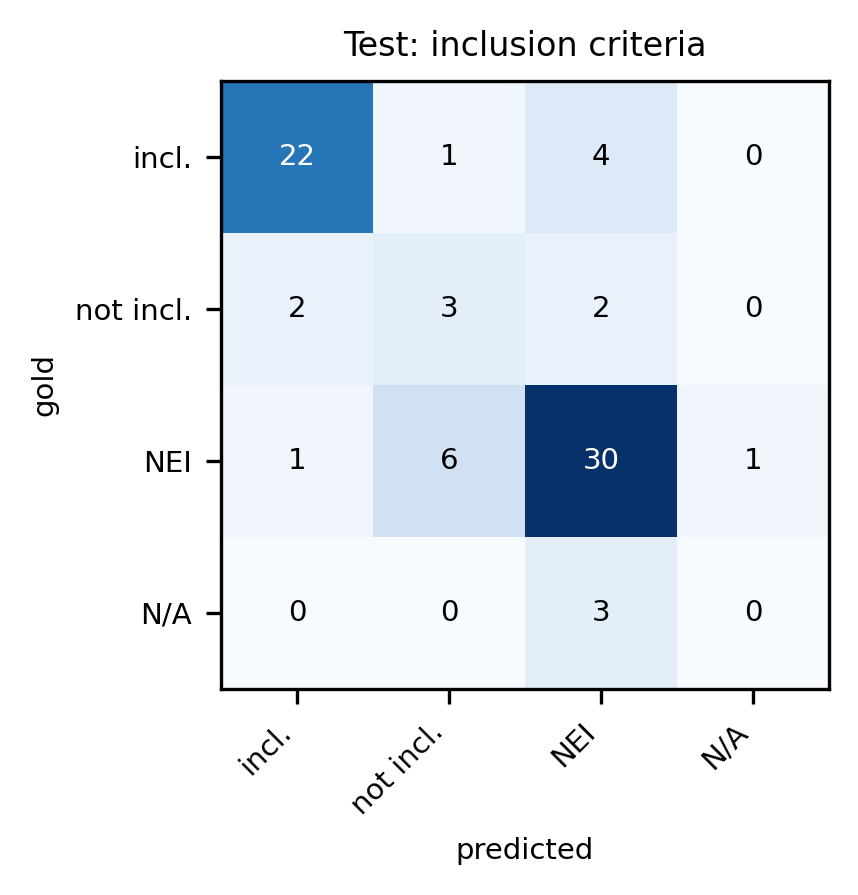
\includegraphics[width=.49\columnwidth]{cm_test_inclusion.png}\hfill
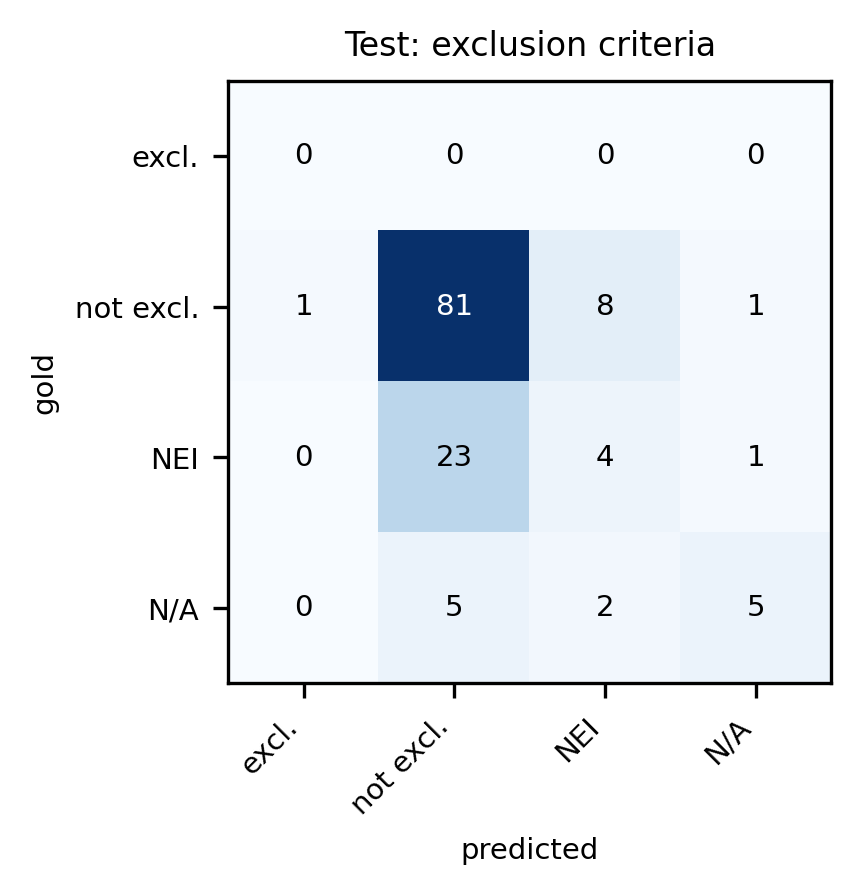
\includegraphics[width=.49\columnwidth]{cm_test_exclusion.png}
\caption{Test confusion matrices for inclusion (left) and exclusion (right). Class imbalance and unknown-to-negative errors remain visible.}\label{fig:cm}\end{figure}

Evidence micro precision/recall/F1 changes from 0.082/0.734/0.147 to 0.437/0.585/0.500. The base model's high recall accompanies many unnecessary citations. Of 206 test rows, 145 have empty expert evidence. Adapted nonempty-gold macro precision/recall/F1 is 0.585/0.656/0.588; empty-gold agreement is 0.876. All-row macro-F1 is 0.791, which would overstate evidence localization if shown without its empty-set convention.

\begin{table*}[t]\centering\caption{Recorded KV benchmark: cached prefill, decode throughput, peak GPU memory, and token equality.}\label{tab:kv}
\begin{tabular}{rrcccccc c}
\hline
In & Out & Unc. tok/s & Cached tok/s & Decode speedup & Prefill ms & Unc. GiB & Cached GiB & Identical \\
\hline
128 & 16 & 23.1 & 26.6 & 1.15 & 43 & 2.97 & 2.93 & yes \\
128 & 64 & 22.8 & 25.9 & 1.14 & 44 & 3.00 & 2.93 & yes \\
128 & 128 & 20.6 & 28.6 & 1.39 & 42 & 3.03 & 2.93 & yes \\
256 & 16 & 12.4 & 29.0 & 2.34 & 63 & 3.04 & 2.97 & yes \\
256 & 64 & 11.8 & 29.2 & 2.48 & 62 & 3.07 & 2.97 & yes \\
256 & 128 & 10.6 & 28.9 & 2.71 & 69 & 3.10 & 2.97 & yes \\
512 & 16 & 6.0 & 28.6 & 4.77 & 139 & 3.18 & 3.05 & yes \\
512 & 64 & 5.7 & 25.7 & 4.54 & 145 & 3.21 & 3.05 & yes \\
512 & 128 & 5.4 & 26.1 & 4.83 & 141 & 3.25 & 3.05 & yes \\
\hline
\end{tabular}
\end{table*}
Table~\ref{tab:kv} shows cached throughput remaining near 26--29 tokens/s while the uncached path slows with longer prefixes. All nine input/output combinations have identical tokens in the saved run. At 512 input and 128 output tokens, cached decode throughput is 4.83 times the reference. Prefill remains dependent on input length, so decode speedup must not be mistaken for end-to-end speedup.

\begin{table*}[t]\centering\caption{Recorded attention benchmark. Memory is extra allocated GPU memory; errors compare tiled output with a reference.}\label{tab:att}
\begin{tabular}{rcccccccc}
\hline
T & Ref ms & Tiled ms & SDPA ms & Ref MiB & Tiled MiB & SDPA MiB & Err fp32 & Err fp16 \\
\hline
256 & 0.54 & 2.30 & 0.10 & 9.0 & 6.0 & 0.8 & 5.4e-07 & 9.6e-04 \\
512 & 1.52 & 5.95 & 0.21 & 36.0 & 6.8 & 1.5 & 6.6e-07 & 9.7e-04 \\
1024 & 5.48 & 19.79 & 0.55 & 144.0 & 8.8 & 3.0 & 5.4e-07 & 9.7e-04 \\
2048 & 17.88 & 69.40 & 0.91 & 576.1 & 11.3 & 6.0 & 6.4e-07 & 9.4e-04 \\
4096 & 69.12 & 273.69 & 4.02 & 2304.2 & 17.3 & 12.0 & 6.0e-07 & 9.3e-04 \\
\hline
\end{tabular}
\end{table*}
At length 4096, Table~\ref{tab:att} shows intermediate memory falling from 2304.2 MiB to 17.3 MiB, but tiled runtime grows from 69.12 to 273.69 ms. SDPA takes 4.02 ms. Small tiles avoid the quadratic score allocation but introduce many Python/kernel dispatches. This result supports memory efficiency, not a speed claim.

\begin{table}[t]\centering\caption{Recorded speculative results for different draft lengths.}\label{tab:spec}
\resizebox{\columnwidth}{!}{\begin{tabular}{rccccccc}
\hline
k & Accept. & Tok/round & s/prompt & Tok/s & Speedup & Peak GiB & Identical \\
\hline
plain & --- & --- & 0.649 & 24.3 & 1.00 & 3.93 & --- \\
1 & 0.81 & 1.76 & 0.894 & 17.6 & 0.73 & 3.93 & 20/20 \\
2 & 0.74 & 2.25 & 0.877 & 18.0 & 0.74 & 3.93 & 20/20 \\
3 & 0.63 & 2.48 & 0.947 & 16.6 & 0.68 & 3.93 & 20/20 \\
4 & 0.63 & 2.86 & 0.985 & 16.0 & 0.66 & 3.93 & 20/20 \\
6 & 0.59 & 3.39 & 1.071 & 14.7 & 0.61 & 3.93 & 20/20 \\
8 & 0.48 & 3.60 & 1.289 & 12.2 & 0.50 & 3.93 & 20/20 \\
\hline
\end{tabular}
}\end{table}
The saved speculation log reports 20/20 matching prompts for every $k$. Plain generation takes 0.649 seconds per prompt and reaches 24.27 tokens/s. For $k=2$, latency rises to 0.877 seconds, throughput falls to 17.96 tokens/s, and acceptance is 0.737. Table~\ref{tab:spec} shows that more accepted tokens per target call do not guarantee lower latency. Draft computation and cache work consume the savings; launch overhead is a plausible explanation, not a directly profiled causal measurement.

\subsection{Eight Representative Errors}
The retained test error analysis identifies 92 rows with label or evidence disagreement. The following eight distinct annotated cases illustrate different symptoms; these are dataset-relative errors, not new clinical adjudications.
\begin{enumerate}
\item Annotation 174, prior axillary surgery: gold unknown becomes not excluded without evidence. Omission is mistaken for a negative history.
\item Annotation 175, chronic renal failure requiring hemodialysis: gold unknown becomes not included. The same missing-information problem affects inclusion.
\item Annotation 177, maintenance hemodialysis: gold not included becomes unknown. Abstention can also lose a benchmark-supported negative decision; its empty gold evidence highlights annotation complexity.
\item Annotation 185, shock/ARDS: gold included becomes unknown. The model fails to connect the cited clinical description to the compound criterion.
\item Annotation 186, heart rate threshold: gold included becomes unknown and cites sentence 3 instead of expert sentence 2. Label and localization fail together.
\item Annotation 307, complex liver-selection criterion: the label remains unknown but five sentences are cited rather than expert sentence 3. Correct classification can coexist with over-retrieval.
\item Annotation 381, age at consent: the label is correct but consent sentence 4 replaces age sentence 0. A related word is insufficient evidence for a numerical condition.
\item Annotation 179, prior central venous procedure: the label matches but the model emits no evidence despite expert sentence 0. A citation-presence rule alone can therefore change a benchmark-correct decision.
\end{enumerate}

\section{Application and Verification}
Figure~\ref{fig:flow} separates raw model output from application review. The Gradio interface accepts synthetic or user-entered notes and criteria, displays evidence and timing, offers three inference modes, and exports Markdown/HTML. The benchmark tab executes decoding and standalone attention comparisons. Input validation rejects empty/oversized notes and invalid criterion counts. HTML output escapes supplied text.

\begin{figure}[t]\centering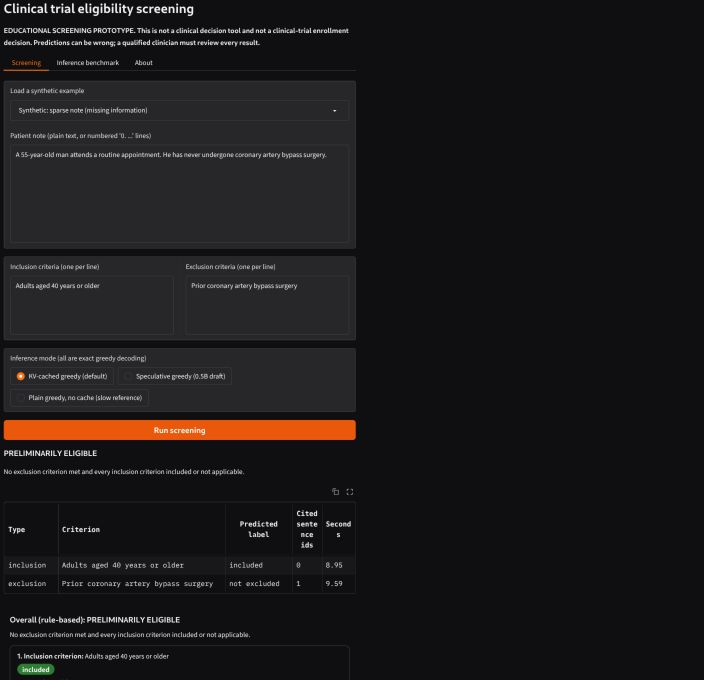
\includegraphics[width=\columnwidth]{application.png}
\caption{Actual browser input view with a synthetic age and explicit negative surgery-history example. The interface exposes the note, criteria, and inference mode.}\label{fig:app}\end{figure}
Figure~\ref{fig:app} illustrates the finalization-stage review layer. Recognized simple age limits with an explicit patient introduction are resolved arithmetically. A decisive prediction with no evidence becomes unknown pending review. Original label/evidence are preserved internally and correction explanations identify original labels. These rules are not retraining, and the metrics in Table~\ref{tab:main} do not measure their effect. They are narrow safeguards: an irrelevant nonempty citation may pass, and relatives' ages or complex criteria can defeat simple parsing.

Aggregation gives priority to excluded or not-included labels, then missing/unparsed results, otherwise preliminary eligibility. It is an explicit rule output without patient-level ground truth. A 20-year-old against a minimum age of 40 produces not included under the supported age rule; unknown surgical history remains unknown.

The current CPU suite passes 113 tests. Finalization corrected a cache API incompatibility by using negative removal counts, and preserved float64 attention for an independent high-precision stress check. Large-logit float32 errors are bounded against a float64 oracle at $10^{-3}$, while float64 algorithm agreement is checked at $10^{-10}$. Ordinary-shape and causal tests retain their existing strict thresholds. These checks do not substitute for new GPU benchmarks, which were not rerun.

\section{Limitations and Conclusion}
The test sample has only eight patients, correlated criterion rows, and an absent gold class. Patient-level confidence intervals and external validation are not provided. Training and prompt-length provenance are incomplete, alternative architectures were not experimentally compared, and prior test evaluations prevent a strict single-final-evaluation claim. Evidence annotations include many empty sets, so conservative application abstention need not improve benchmark accuracy. CPU inference can be slow, custom decoders are batch-one, and UI truncation/sentence splitting have edge cases.

The system nevertheless demonstrates a complete criterion-to-evidence workflow and separately testable inference mechanisms. LoRA improves this benchmark over the base and majority baselines, caching accelerates recorded long-prefix decoding, and online softmax reduces attention memory. Speculation correctly preserves saved greedy outputs while remaining slower. Further work should focus on validation-only reasoning probes, calibrated abstention, stronger evidence verification, and complete experiment provenance before broader use.

\appendices
\section{Reproducibility and AI Assistance}
The repository includes training configurations, prediction JSONL, split manifest, benchmark logs, tests, and report sources. Reproduction and demonstration instructions are in \texttt{docs/REPRODUCIBILITY.md} and \texttt{docs/DEMO\_SCRIPT.md}. Weights are hosted at \url{https://huggingface.co/AK302/trialgpt-qwen1.5b-lora}, subfolder \texttt{lora\_r16\_bal/epoch3}. Source: \url{https://github.com/AaizUrRehmanKazmi/Transformers}.

The existing repository acknowledges Claude assistance with scaffolding/debugging. Codex assisted with repository review, application review rules, cache compatibility, numerical tests, literature lookup, and this report draft. Recorded experiments are distinguished from tests executed during finalization. The student must verify authorship details, review the paper, record the demonstration, and understand and defend all submitted code. This appendix describes assistance rather than claiming independent student verification that has not been confirmed.

\begin{thebibliography}{9}
\bibitem{trialgpt} Q. Jin et al., ``Matching patients to clinical trials with large language models,'' \emph{Nature Communications}, vol. 15, art. 9074, 2024, doi: 10.1038/s41467-024-53081-z.
\bibitem{attention} A. Vaswani et al., ``Attention is all you need,'' 2017. \url{https://arxiv.org/abs/1706.03762}.
\bibitem{lora} E. J. Hu et al., ``LoRA: Low-rank adaptation of large language models,'' 2021. \url{https://arxiv.org/abs/2106.09685}.
\bibitem{flash} T. Dao et al., ``FlashAttention: Fast and memory-efficient exact attention with IO-awareness,'' 2022. \url{https://arxiv.org/abs/2205.14135}.
\bibitem{spec} Y. Leviathan, M. Kalman, and Y. Matias, ``Fast inference from transformers via speculative decoding,'' \emph{ICML}, PMLR 202, pp. 19274--19286, 2023.
\bibitem{qwen} Qwen Team, ``Qwen2.5-1.5B-Instruct model card.'' \url{https://huggingface.co/Qwen/Qwen2.5-1.5B-Instruct}. Accessed Nov. 7, 2026.
\bibitem{smol} Hugging Face, ``SmolLM2-1.7B-Instruct model card.'' \url{https://huggingface.co/HuggingFaceTB/SmolLM2-1.7B-Instruct}. Accessed Nov. 7, 2026.
\bibitem{smolconfig} Hugging Face, ``SmolLM2-1.7B-Instruct configuration,'' \texttt{config.json}, model repository, accessed Nov. 7, 2026.
\bibitem{draft} Qwen Team, ``Qwen2.5-0.5B-Instruct model card.'' \url{https://huggingface.co/Qwen/Qwen2.5-0.5B-Instruct}. Accessed Nov. 7, 2026.
\end{thebibliography}
\end{document}
